\documentclass[[12pt,twoside]{book}
\usepackage{_my_document_style}
\begin{document}
%
\begin{myExampleX}{Zero lift angle of a finite wing (graphic method)}{\ding{46}\ \myIconGraph\ }% \ \Keyboard\ %
\label{example:Zero:Lift:Angle:Graphic:Method}
%
\def\mySpanWingMT{26.800000}
\def\myMach{0.700000}
\def\myAspectRatioWing{7.108753}
\def\myChordRootWingMT{5.200000}
\def\myChordTipWingMT{2.340000}
\def\mySweepLEWingDEG{27.500000}
\def\mySweepLEWingRAD{0.479966}
\def\mySweepQuarterChordWingDEG{24.059464}
\def\mySweepQuarterChordWingRAD{0.419917}
\def\myCoeffAChordWing{-0.213433}
\def\myCoeffBChordWingMT{5.200000}
\def\myAlphaZeroLiftRootWingDEG{-3.000000}
\def\myAlphaZeroLiftTipWingDEG{-1.500000}
\def\myAlphaZeroLiftRootWingRAD{-0.052360}
\def\myAlphaZeroLiftTipWingRAD{-0.026180}
\def\myTaperRatioWing{0.450000}
\def\myTwistWingDEG{-1.500000}
\def\myTwistWingRAD{-0.026180}
\def\myTwistWingDEG{0.450000}
\def\myAreaWingMTsquared{101.036000}
\def\myCoeffAAeroTwistWingRADMT{0.001954}
\def\myCoeffATwistWingRADMT{-0.001954}
\def\myCoeffBAeroTwistWingRAD{-0.052360}
\def\myThicknessOverChordTipWing{0.090000}
\def\myThicknessOverChordRootWing{0.150000}
\def\myThicknessOverChordMeanWing{0.123793}
\def\myCoeffAPercThicknessWingMT{-0.004478}
\def\myCoeffBPercThicknessWing{0.150000}
\def\myAlphaZeroLiftMeanWingRAD{-0.040925}
\def\myAlphaZeroLiftMeanWingDEG{-0.040925}
\def\myAlphaZeroLiftDatcomWingRAD{-0.026308}
\def\myAlphaZeroLiftDatcomWingDEG{-1.507328}
\def\myAlphaZeroLiftWingRAD{-0.029490}
\def\myAlphaZeroLiftWingDEG{-1.689655}
\def\myDeltaAlphaZeroLiftOverTwistWing{-0.381000}
\def\myPrandtlGlauertCorrectionAlphaZeroLiftWing{0.850000}

%
\noindent
Let us consider again the wing of the example~\ref{example:Geometric:Characteristics:Of:A:Straight:And:Tapered:Wing} having straight leading and trailing edges, wingspan $b=\SI[round-precision=1]{\mySpanWingMT}{\metre}$,root chord $c_\mathrm{r}=\SI[round-precision=2]{\myChordRootWingMT}{\metre}$,
tip chord $c_\mathrm{t}=\SI[round-precision=2]{\myChordTipWingMT}{\metre}$
and leading edge sweep angle $\Lambda_\mathrm{le}=\SI[round-precision=1]{\mySweepLEWingDEG}{\deg}$.
Furthermore, the root profile has a zero lift angle
$\alpha_{0\ell,\mathrm{r}}=\SI[round-precision=1]{\myAlphaZeroLiftRootWingDEG}{\deg}$
while the tip profile has a zero lift angle
$\alpha_{0\ell,\mathrm{t}}=\SI[round-precision=1]{\myAlphaZeroLiftTipWingDEG}{\deg}$,
with twist angle
$\epsilon_{\mathrm{g,t}}=\SI[round-precision=1]{\myTwistWingDEG}{\deg}$.
Lastly, the flight Mach number is $\Mach=\SI[round-precision=2]{\myMach}{}$.

We want to calculate the zero lift angle of the wing $\alpha_{0L}$ 
according to the semiempirical formula
\begin{equation}
\label{eq:Wing:Alpha:Zero:Lift:Roskam:Datcom}
\alpha_{0L} =
  \Big(
    \bar{\alpha}_{0\ell} + K_{\alpha,1} \, \epsilon_{\mathrm{g,t}}
  \Big) 
  \, K_{\alpha,2}
\end{equation}
In this modeling
\[
\bar{\alpha}_{0\ell} = \frac{2}{S} \int_0^{b/2} \alpha_{0\ell}(Y)\, c(Y) \diff{Y}
\]
is the mean value of the section zero lift angle.
The coefficient
$K_{\alpha,1}$ is the ratio
$\upDelta\alpha_{0L}/\epsilon_{\mathrm{g,t}}$ which we can read from
figure~\ref{fig:Wing:DalphaZeroLift:Roskam:Plots},
function of the sweep angle $\Lambda_{c/4}$, of the aspect ratio $\AR$
and of the taper ratio $\lambda$.
The coefficient
$K_{\alpha,2}$ is a correction factor due to any
effects of compressibility, it can be read from figure~\ref{fig:Alpha:Zero:Lift:PrandtlGlauert:Scale:Plots}
and it is a function of the flight Mach number, i.e. of the product $\Mach\cos\Lambda_{c/4}$,
and the average value of the per cent thickness of the profiles $\overline{(t/c)}$.
%\[
%\overline{(t/c)}
%  = \frac{2}{S} \int_0^{b/2} \left(\frac{t}{c}\right)(Y)\, c(Y) \diff{Y}
%\]

\medskip

The laws of variation along the wingspan must be reconstructed:%
\begin{inparaenum}[(\itshape i\normalfont)]
\item
of the chord,
\item
of the zero lift angle of section,
\item
of the percentage of section thickness.
\end{inparaenum}
In the absence of specific indications, it can be assumed
that the last two laws are linear.

In the example~\ref{example:Geometric:Characteristics:Of:A:Wing:With:Sweep:Angle:Not:Null}, as regards the chords, it was found that
\[
A_c
  = \mathunderline{mydarkblue}{ \SI[round-precision=3]{\myCoeffAChordWing}{} }
\;,\quad
B_c
  = \mathunderline{mydarkblue}{ \SI[round-precision=2]{\myCoeffBChordWingMT}{\metre} }
\]
and
\[
c \big( Y \big) = A_c \, Y + B_c
  = \SI[round-precision=3]{\myCoeffAChordWing}{} \, Y
    + \SI[round-precision=2]{\myCoeffBChordWingMT}{\metre}
\]

The linear law holds for the  zero lift angles of section $\alpha_{0\ell} \big( Y \big) = A_{\alpha} \, Y + B_{\alpha}$ 
with
\[
A_{\alpha}
  = \frac{\alpha_{0\ell,\mathrm{t}} - \alpha_{0\ell\mathrm{r}}}{b/2}
  = 
    2 \frac{
      \SI[round-precision=4]{\myAlphaZeroLiftTipWingRAD}{\radian} 
        - ( \SI[round-precision=4]{\myAlphaZeroLiftRootWingRAD}{\radian} )
    }{
      \SI[round-precision=2]{\mySpanWingMT}{\metre}
    }
  = \mathunderline{mydarkblue}{ \SI[round-precision=5]{\myCoeffAAeroTwistWingRADMT}{\radian/\metre} }
\]
\[
B_{\alpha}
  = \alpha_{0\ell,\mathrm{r}}
  = \mathunderline{mydarkblue}{ \SI[round-precision=4]{\myAlphaZeroLiftRootWingRAD}{\radian} }
\]
therefore
\[
\alpha_{0\ell} \big( Y \big) = A_{\alpha} \, Y + B_{\alpha}
  = (\SI[round-precision=5]{\myCoeffAAeroTwistWingRADMT}{\radian/\metre}) \, Y
    \SI[round-precision=4]{\myAlphaZeroLiftRootWingRAD}{\radian}
\]

The law of the percentage thickness of the profiles is obtained similarly,
imposing
$(t/c)\,\big( Y \big) = A_{t/c} \, Y + B_{t/c}$ 
wiht
\[
A_{t/c}
  = \frac{(t/c)_{\mathrm{t}} - (t/c)_{\mathrm{r}}}{b/2}
  = 
    2 \frac{
      \SI[round-precision=2]{\myThicknessOverChordTipWing}{} 
        - \SI[round-precision=4]{\myThicknessOverChordRootWing}{}
    }{
      \SI[round-precision=2]{\mySpanWingMT}{\metre}
    }
  = \mathunderline{mydarkblue}{ \SI[round-precision=5]{\myCoeffAPercThicknessWingMT}{\metre^{-1}} }
\]
\[
B_{t/c}
  = (t/c)_{\mathrm{r}}
  = \mathunderline{mydarkblue}{ \SI[round-precision=2]{\myCoeffBPercThicknessWing}{} }
\]
therefore
\[
(t/c)\,\big( Y \big) = A_{t/c} \, Y + B_{t/c}
  = (\SI[round-precision=5]{\myCoeffAPercThicknessWingMT}{\metre^{-1}}) \, Y
    + \SI[round-precision=2]{\myCoeffBPercThicknessWing}{}
\]

The assigned wing has a taper ratio
\[
\lambda
  =\frac{c_\mathrm{t}}{c_\mathrm{r}}
  =\frac{\SI[round-precision=2]{\myChordTipWingMT}{\metre}}{\SI[round-precision=2]{\myChordRootWingMT}{\metre}}
  =\mathunderline{mydarkblue}{ \SI[round-precision=2]{\myTaperRatioWing}{} }
\]
a wing surface
\[
\begin{split}
S & {}= \frac{b}{2} \, c_\mathrm{r} \, \big( 1 + \lambda \big) \\
  & {}=
    \num{0.5} \cdot \SI[round-precision=1]{\mySpanWingMT}{\metre}
      \cdot \SI[round-precision=2]{\myChordRootWingMT}{\metre}
      \cdot \big( 1 + \SI[round-precision=2]{\myTaperRatioWing}{} \big) 
    = \mathunderline{mydarkblue}{ \SI[round-precision=1]{\myAreaWingMTsquared}{\metre^2} }
\end{split}
\]
an aspect ratio
\[
\AR
  = \frac{b^2}{S}
  = \frac{\big(\SI[round-precision=1]{\mySpanWingMT}{\metre}\big)^2}{\SI[round-precision=1]{\myAreaWingMTsquared}{\metre^2}}
  = \mathunderline{mydarkblue}{ \num[round-precision=2]{\myAspectRatioWing} }
\]
and a sweep angle
\[
\tan
\Lambda_{c/4}
   = \tan (\SI[round-precision=3]{\mySweepLEWingRAD}{\radian})
      - \dfrac{
         \num[round-precision=2]{1.0}
         \cdot (1-\SI[round-precision=2]{\myTaperRatioWing}{})
      }{
         \num[round-precision=2]{\myAspectRatioWing}
         \cdot (1+\SI[round-precision=2]{\myTaperRatioWing}{})} 
   \quad
   \Rightarrow
   \quad
   \Lambda_{c/4}
      = \mathunderline{mydarkblue}{ \SI[round-precision=3]{\mySweepQuarterChordWingRAD}{\radian} }
      = \mathunderline{mydarkblue}{ \SI[round-precision=1]{\mySweepQuarterChordWingDEG}{\deg} }
\]

At this point it is possible to calculate the average values
\[
\begin{split}
\bar{\alpha}_{0\ell} 
  & {}= \frac{2}{S} \int_0^{b/2} \alpha_{0\ell}(Y)\, c(Y) \diff{Y}
    = \frac{2}{S} \int_0^{b/2} 
      \Big( A_{\alpha} \, Y + B_{\alpha} \Big)\, \Big( A_c Y + B_c \Big)
        \diff{Y}
\\[2pt]
  & ={}
    \frac{2}{ \SI[round-precision=1]{\myAreaWingMTsquared}{\metre^2} }
    \int_{\SI{0}{m}}^{
      \calcSI[round-precision=1,fixed-exponent=0,scientific-notation=fixed]{0.5*\mySpanWingMT}{\metre}
    }
    \Big( 
      \SI[round-precision=5]{\myCoeffAAeroTwistWingRADMT}{\radian/\metre} \; Y
        \SI[round-precision=4]{\myAlphaZeroLiftRootWingRAD}{\radian}
    \Big) 
    \Big( 
      \SI[round-precision=3]{\myCoeffAChordWing}{} \; Y
        + \SI[round-precision=2]{\myCoeffBChordWingMT}{\metre}
    \Big) \diff{Y}
\\[4pt]
  & {}= \mathunderline{mydarkblue}{ \SI[round-precision=4]{\myAlphaZeroLiftMeanWingRAD}{\radian} }
  = \mathunderline{mydarkblue}{ \SI[round-precision=2]{\myAlphaZeroLiftMeanWingDEG}{\deg} }
\end{split}
\]

\[
\begin{split}
\overline{(t/c)} & {}= \frac{2}{S} \int_0^{b/2} (t/c)\big(Y\big)\, c\big(Y\big) \diff{Y}
  = \frac{2}{S} \int_0^{b/2} 
    \Big( A_{t/c} \, Y + B_{t/c} \Big)\, \Big( A_c Y + B_c \Big)
      \diff{Y}
\\[2pt]
  & ={}
    \frac{2}{ \SI[round-precision=1]{\myAreaWingMTsquared}{\metre^2} }
    \int_{\SI{0}{m}}^{
      \calcSI[round-precision=1,fixed-exponent=0,scientific-notation=fixed]{0.5*\mySpanWingMT}{\metre}
    }
    \Big( 
      \SI[round-precision=5]{\myCoeffAPercThicknessWingMT}{\metre^{-1}} \; Y
        + \SI[round-precision=3]{\myCoeffBPercThicknessWing}{}
    \Big) 
    \Big( 
      \SI[round-precision=3]{\myCoeffAChordWing}{} \; Y
        + \SI[round-precision=2]{\myCoeffBChordWingMT}{\metre}
    \Big) \diff{Y}
\\[4pt]
  & {}= \mathunderline{mydarkblue}{ \SI[round-precision=3]{\myThicknessOverChordMeanWing}{} }
\end{split}
\]

With the values thus obtained, from figure~\ref{fig:Wing:DalphaZeroLift:Roskam:Plots}
we can derive
\[
\Lambda_{c/4}=\SI[round-precision=1]{\mySweepQuarterChordWingDEG}{\deg}\;,\;\,
\AR=\num[round-precision=2]{\myAspectRatioWing}\;,\;\,
\lambda=\SI[round-precision=2]{\myTaperRatioWing}{}
%
%\quad \Longrightarrow \quad
%\quad \begin{array}{@{}c@{}} \myIconGraph \\[-4pt] \Longrightarrow \end{array} \quad
\adjustbox{center=4em}{%
  \adjustbox{lap=\width}{\raisebox{2.2ex}[0pt][0pt]{\myIconGraph}}$\Longrightarrow$%
}
%
K_{\alpha,1} =
  \frac{\upDelta\alpha_{0L}}{\epsilon_{\mathrm{g,t}}}
  = \mathunderline{mydarkblue}{ \SI[round-precision=3]{\myDeltaAlphaZeroLiftOverTwistWing}{} }
\]
and
from figure~\ref{fig:Alpha:Zero:Lift:PrandtlGlauert:Scale:Plots}
we can obtain
\[
\Mach \cos \Lambda_{c/4}=
  \calcSI[round-precision=2,fixed-exponent=0,scientific-notation=fixed]{
    \myMach * cos(\mySweepQuarterChordWingRAD)
  }{}\;,\;\,
\overline{(t/c)} =
  \SI[round-precision=3]{\myThicknessOverChordMeanWing}{}
%
%\quad \Longrightarrow \quad
%\quad \begin{array}{@{}c@{}} \myIconGraph \\[-4pt] \Longrightarrow \end{array} \quad
\adjustbox{center=4em}{%
  \adjustbox{lap=\width}{\raisebox{2.2ex}[0pt][0pt]{\myIconGraph}}$\Longrightarrow$%
}
%
K_{\alpha,2} =
  \frac{\alpha_{0L}}{\alpha_{0L}\big|_{\Mach=\num{0.3}}} 
  = \mathunderline{mydarkblue}{ \SI[round-precision=2]{\myPrandtlGlauertCorrectionAlphaZeroLiftWing}{} }
\]

Therefore, the wing assigned, at the specified Mach number, has a zero lift angle
\[
\begin{split}
\label{eq:Wing:Alpha:Zero:Lift:Roskam:Datcom}
\alpha_{0L} 
  & {}=
    \Big(
      \bar{\alpha}_{0\ell} + K_{\alpha,1} \, \epsilon_{\mathrm{g,t}}
    \Big) \, K_{\alpha,2}
\\
  & {}= 
    \Big(
      \SI[round-precision=4]{\myAlphaZeroLiftMeanWingRAD}{\radian}
        + ( \SI[round-precision=3]{\myDeltaAlphaZeroLiftOverTwistWing}{} )
          ( \SI[round-precision=4]{\myTwistWingRAD}{\radian} )
    \Big)
      \cdot \SI[round-precision=2]{\myPrandtlGlauertCorrectionAlphaZeroLiftWing}{}
\\[4pt]
  & {}= \mathunderline{mydarkblue}{ \SI[round-precision=4]{\myAlphaZeroLiftDatcomWingRAD}{\radian} }
  = \mathunderline{mydarkblue}{ \SI[round-precision=2]{\myAlphaZeroLiftDatcomWingDEG}{\deg} }
\end{split}
\]
According to the modeling introduced here
this value of the zero lift angle of the wing is linked to the particular value of the flight Mach number. For a product $\Mach \cos\Lambda_{c/4}$ sufficiently high
$\alpha_{0L}$ it will vary as the Mach number changes due to the compressibility correction factor $K_{\alpha,2}$.

The zero lift angle calculated with the formula
of the example~\ref{example:Zero:Lift:Angle:Of:A:Finite:Wing}
is
\[
\alpha_{0L} 
  = \frac{2}{S} \int_0^{b/2} 
    \Big[ 
      \alpha_{0\ell}\big(Y\big) - \epsilon_\mathrm{g}\big(Y\big) 
    \Big] \, c(Y) \diff{Y}
  = \mathunderline{mydarkblue}{ \SI[round-precision=4]{\myAlphaZeroLiftWingRAD}{\radian} }
  = \mathunderline{mydarkblue}{ \SI[round-precision=2]{\myAlphaZeroLiftWingDEG}{\deg} }
\]
\begin{figure}[H]%[!htbp]
  %\centering
  %\checkoddpage
  %\centering
  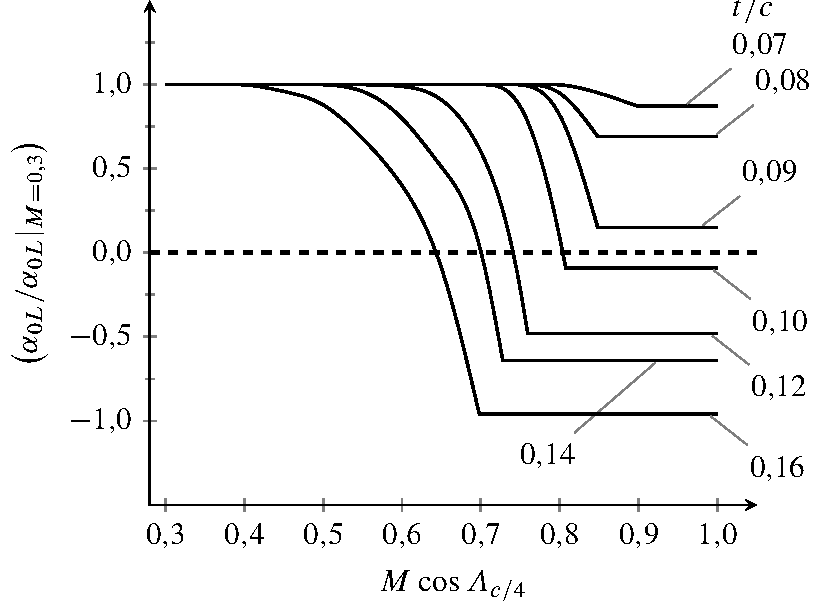
\includegraphics[width=0.65\textwidth]{Chapter_2/zero_lift_angle_graphic_method/plot_alpha0_PrandtlGlauert_scale.pdf}%
  \caption{\finalhyphendemerits=1000
           Correction factor 
           \smash{$\big(\alpha_{0L}\mathlarger{/}\alpha_{0L}|_{\Mach=\num[round-precision=1]{0.3}}\big)$}
           which incorporates the effects of compressibility for the calculation of the zero lift angle
          of a finite wing $\alpha_{0L}$.}
  \label{fig:Alpha:Zero:Lift:PrandtlGlauert:Scale:Plots}%
\end{figure}
\end{myExampleX}

\EnlargedFigureX% needs two latex passes
  {p}% #1: t, b, p
  {%
    \centering
    \begin{tabular} {@{}c@{}}
      \subfloat%\subfigure
          [%
          ]%
          {\label{fig:Wing:DalphaZeroLift:Roskam:Plots:A}%
		      \includegraphics%
		        %[width=0.52\textwidth]%
		        % [height=5.5cm]%
		        [width=0.52\textwidth]%
		        {Chapter_2/zero_lift_angle_graphic_method/plot_Dalpha0_over_epsT_lam0.pdf}%
          }%
      \\
      \subfloat%\subfigure
          [%
          ]%
          {\label{fig:Wing:DalphaZeroLift:Roskam:Plots:B}%
		      \includegraphics%
		        %[width=0.52\textwidth]%
		        % [height=5.5cm]%
		        [width=0.52\textwidth]%
		       {Chapter_2/zero_lift_angle_graphic_method/plot_Dalpha0_over_epsT_lam05.pdf}%
          }%
      \\
      \subfloat%\subfigure
          [%            
          ]%
          {\label{fig:Wing:DalphaZeroLift:Roskam:Plots:C}%
		      \includegraphics%
		        %[width=0.52\textwidth]%
		        % [height=5.5cm]%
		        [width=0.52\textwidth]%
		       {Chapter_2/zero_lift_angle_graphic_method/plot_Dalpha0_over_epsT_lam1.pdf}%
          }%
    \end{tabular}
  }
  {\finalhyphendemerits=1000
      Correction factor \smash{$\big(\upDelta\alpha_{0L}/\epsilon_\mathrm{t}\big)$} for the calculation of the zero lift angle of a finite wing $\alpha_{0L}$.%
   }  
   {fig:Wing:DalphaZeroLift:Roskam:Plots}%% #4: the label
\end{document}